\subsection{Dijets of light and heavy flavors (Doga)}


\begin{figure}[h]
\begin{center}
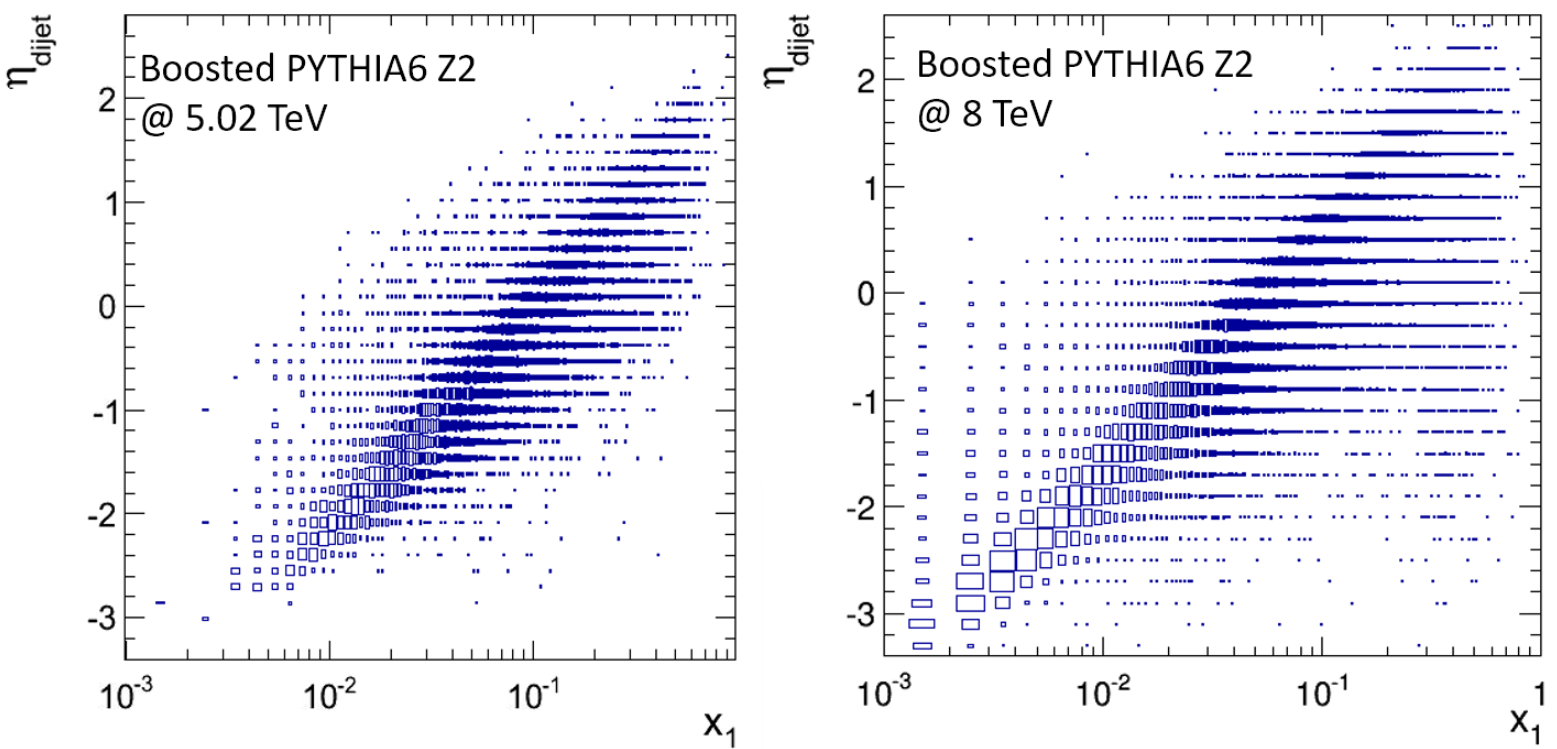
\includegraphics[width= 0.9\textwidth]{figures/x_vs_eta.png}
\caption{}
\label{fig:dijetCorr}
\end{center}
\end{figure}

The measurement of dijet pseudorapidity distributions were shown to be sensitive to nPDF effects \cite{}, such that it can discriminate between different nPDF sets, by the earlier pPb measurement at 5.02 TeV \cite{}. The tight correlation shown in Fig. \ref{fig:dijetCorr} between dijet $\eta_{dijet} = \eta_{1} + \eta_{2}$ and parton x from Pb nuclei is the underlying reason of the sensitivity to nPDF. At 8 TeV the slope of the correlation changes as $x \approx 1/\sqrt{s_{\rm NN}}$. This allows us to push the boundaries of x regions without changing the $\eta$ range used in the analyses. Moreover, with the increase in di-b-jet cross section at 8 TeV. It will be possible to repeat the measurement of $\eta_{dijet}$ distributions where both leading and subleading jets are tagged as b-jets. As $96\%$ of di-b-jet production is gluon fusion processes, this measurement is almost entirely measurement of gluon nPDF.


Different x values can be probed by selecting on $\eta_{dijet}$, while different $Q$ values can be chosen by applying requirements on $\pt^{\rm ave} = (p_{\rm T,1} + p_{\rm T,2})/2$, which is directly correlated to $Q$. The reach on x-Q plane is calculated by parametrizing the $x_{\rm Pb}$ distributions in boosted {\sc pythia} for a specific $\eta_{dijet}$ and $\pt^{\rm ave}$ selections. An example case is shown in Fig. \ref{fig:distX}. The area under the gaussian curves that are left outside of a cut around the mean $log(x)$ value given by $\mu$ of the gaussian fit is scaled with the total number of events. The region of sensitivity is calculated by when the number of events outside of this range on either side of the mean, given as $0.5 \times ErfcInverse((x-\mu)/(\sqrt{2}\sigma))$, falls below $1/\epsilon_{\rm stat}^{2}$. The same procedure is applied in $Q$. The reach in x and Q are calculated in several bins of $\eta_{dijet}$ and $\pt^{\rm ave}$ and overlaid as patches of areas on x-Q plane. The results are shown in Figs. \ref{fig:xQscanBjet} and \ref{fig:xQscanInclusive}.

\begin{figure}[h]
\begin{center}
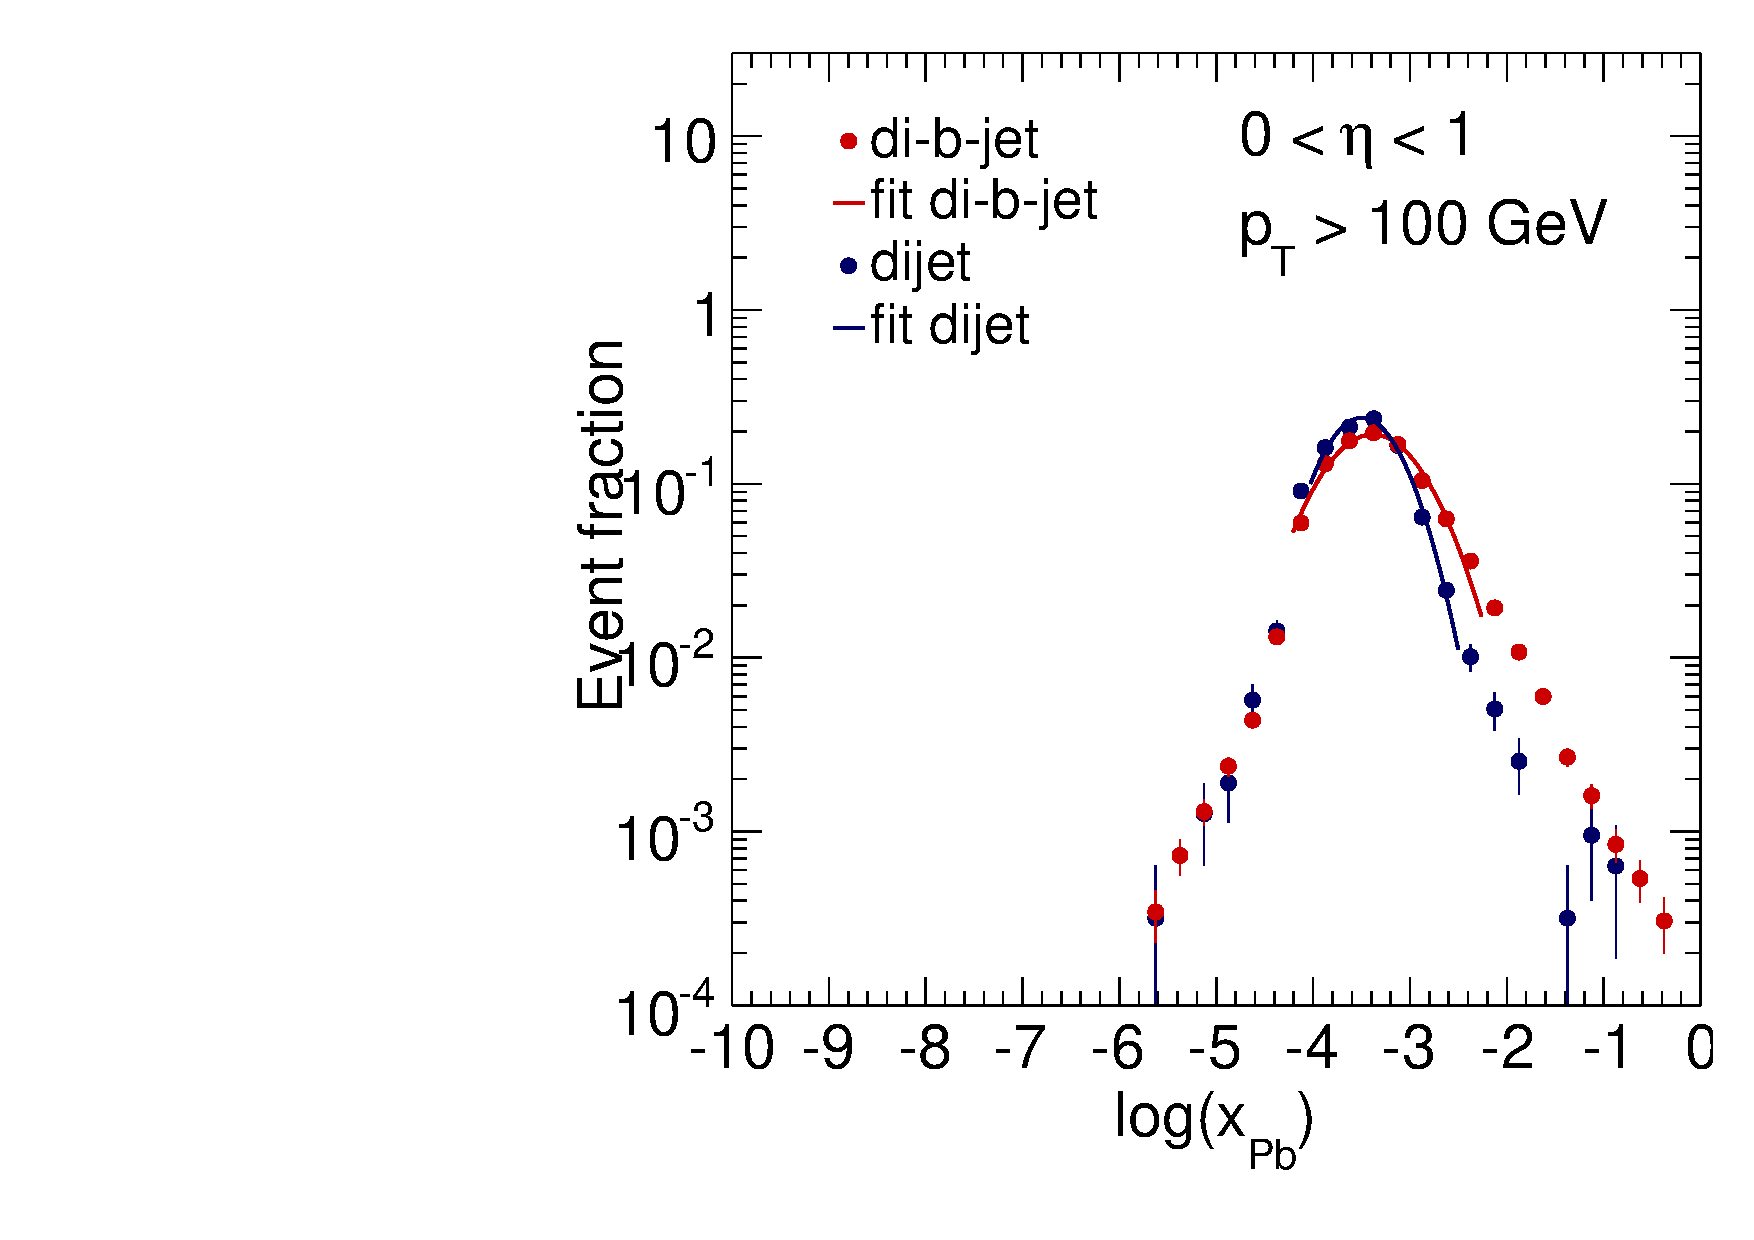
\includegraphics[width= 0.4\textwidth]{figures/DistCompareBJetInclusive.pdf}
\caption{}
\label{fig:distX}
\end{center}
\end{figure}

The resulting x-Q scan for di-b-jet processes are shown in Fig. \ref{xQscanBjet} and with $100$ nb$^{-1}$, it will be possible to provide constraints for $x < 3-4 \times 10^{-3}$, which has no data constraints \cite{}.

\begin{figure}[h]
\begin{center}
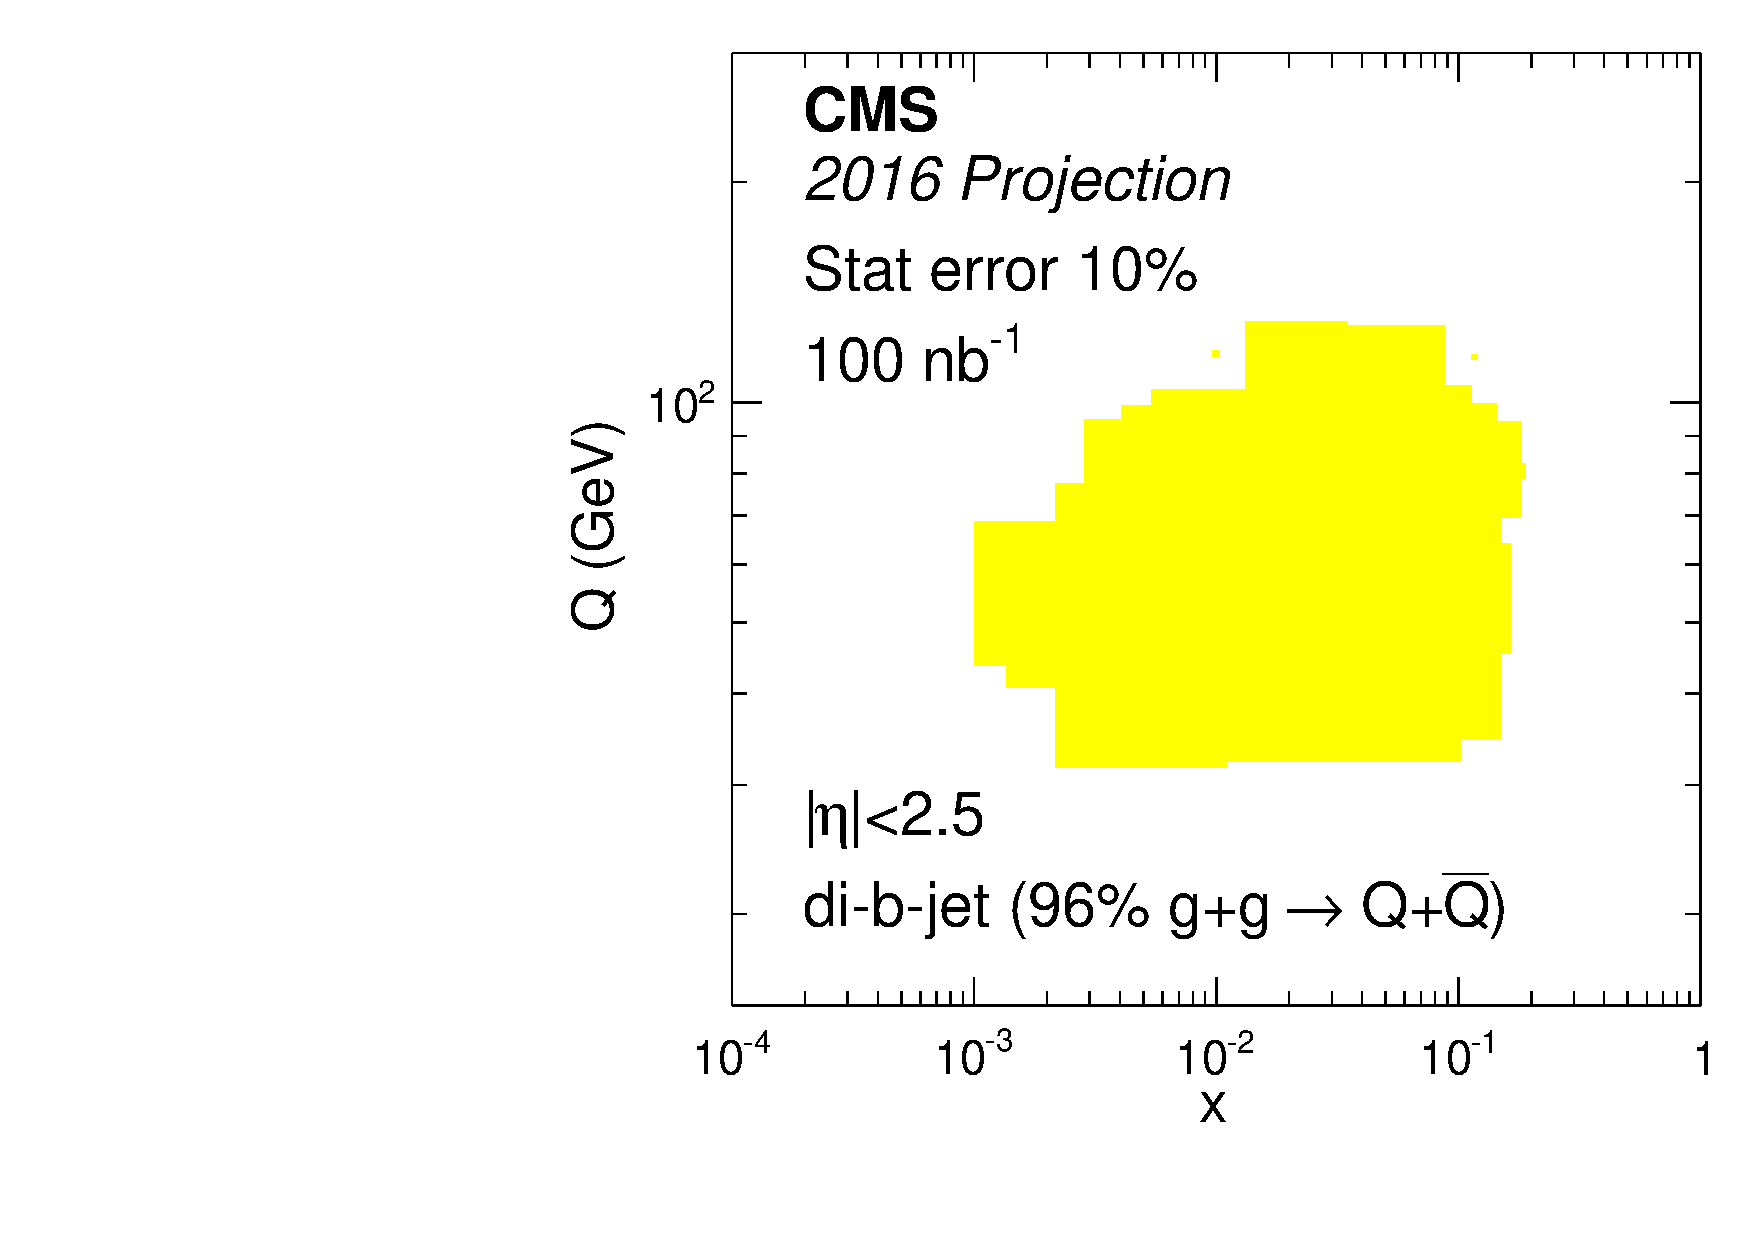
\includegraphics[width= 0.4\textwidth]{figures/filledQX_Lumi100_BJet.pdf}
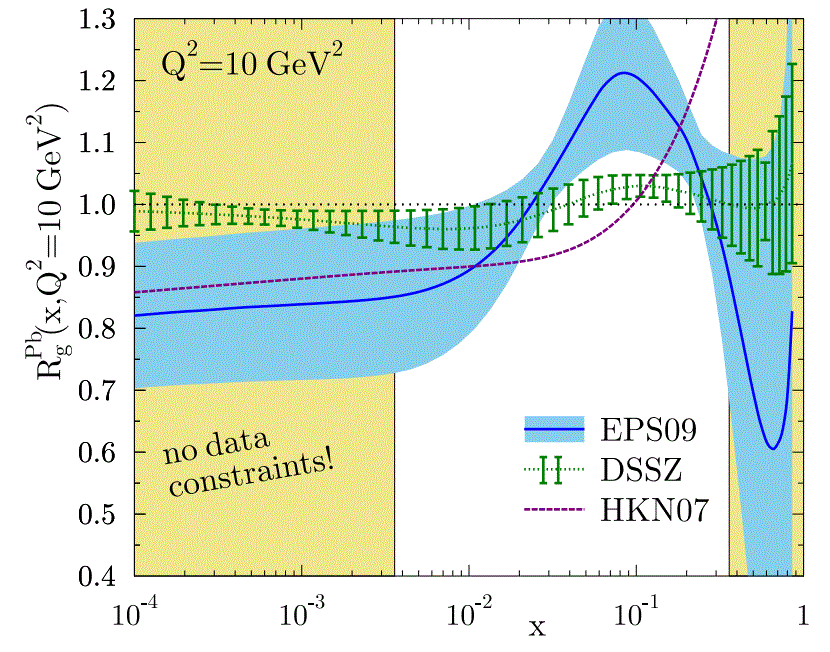
\includegraphics[width= 0.45\textwidth]{figures/eps09_10GeV_Gluon_nPDF.png}
\caption{}
\label{fig:xQscanBjet}
\end{center}
\end{figure}

Although, inclusive flavor dijet measurement has significant contribution from $f + g \rightarrow f + g$ ($39 \%$) in addition to gluon fusion ($54 \%$), and is therefore not a pure handle on gluon nPDF, which is less constrained compared to quark nPDF, they are still of great interest as they are produced in copious amounts and their sensitivity extends over a much larger x-Q range. The x reach of b-jet measurement is limited by the $\eta$ coverage of the tracker, i.e. $|\eta| < 2.5$. However, the untagged flavor jet measurements can be extended up to $\eta = 3$ with good control on systematics and up to $\eta = 5$ if the luminosity allows one to calibrate the energy response Hadronic Forward (HF) calorimeter. The x-Q span of inclusive dijet measurement is shown in Fig. \ref{fig:xQscanInclusive} for the two pseudorapidity selections for a measurement with better than $3\%$ statistical precision. The statistical uncertainty as a function of x in the high $x$ region is shown in Fig. \ref{fig:XreachWithPseudorapidity} for different luminosity scenarios, 10, 25, 50 and 100 $nb^{-1}$, on the left panel for $|\eta| < 3$ and on the middle for $|\eta| < 5$. For dijets selected within $|\eta| < 3$, where good systematic precision can be provided, the $x$ reach benefits from a higher luminosity 8 TeV data. It is possible to measure up to $x = 0.6$ within $10 \%$ statistical uncertainty with 100 $nb^{-1}$ pPb data. 

For $|\eta| < 5$ selection, the statistical uncertainty is no longer the dominant factor on the precision of the measurement as systematic uncertainties caused by the jet energy scale uncertainties in HF become more significant at HF. It is possible to reduce the systematic uncertainties by applying data-driven methods to calibrate HF, but for that a high luminosity data sample is needed. The improvement in the errors on data-driven response corrections in 7 and 8 TeV pp data are shown on the right panel of Fig. \ref{fig:XreachWithPseudorapidity}. Even with $36$ pb$^{-1}$ pp data the uncertainty on corrections in HF is $\approx 10 \%$. The uncertainty on these corrections shrink to $4\%$ only with a luminosity of $20$ fb$^{-1}$. Therefore, it will only be possible to probe high $x$ values that are sensitive to a very interesting range of nPDF modifications with high luminosity data.

\begin{figure}[h]
\begin{center}
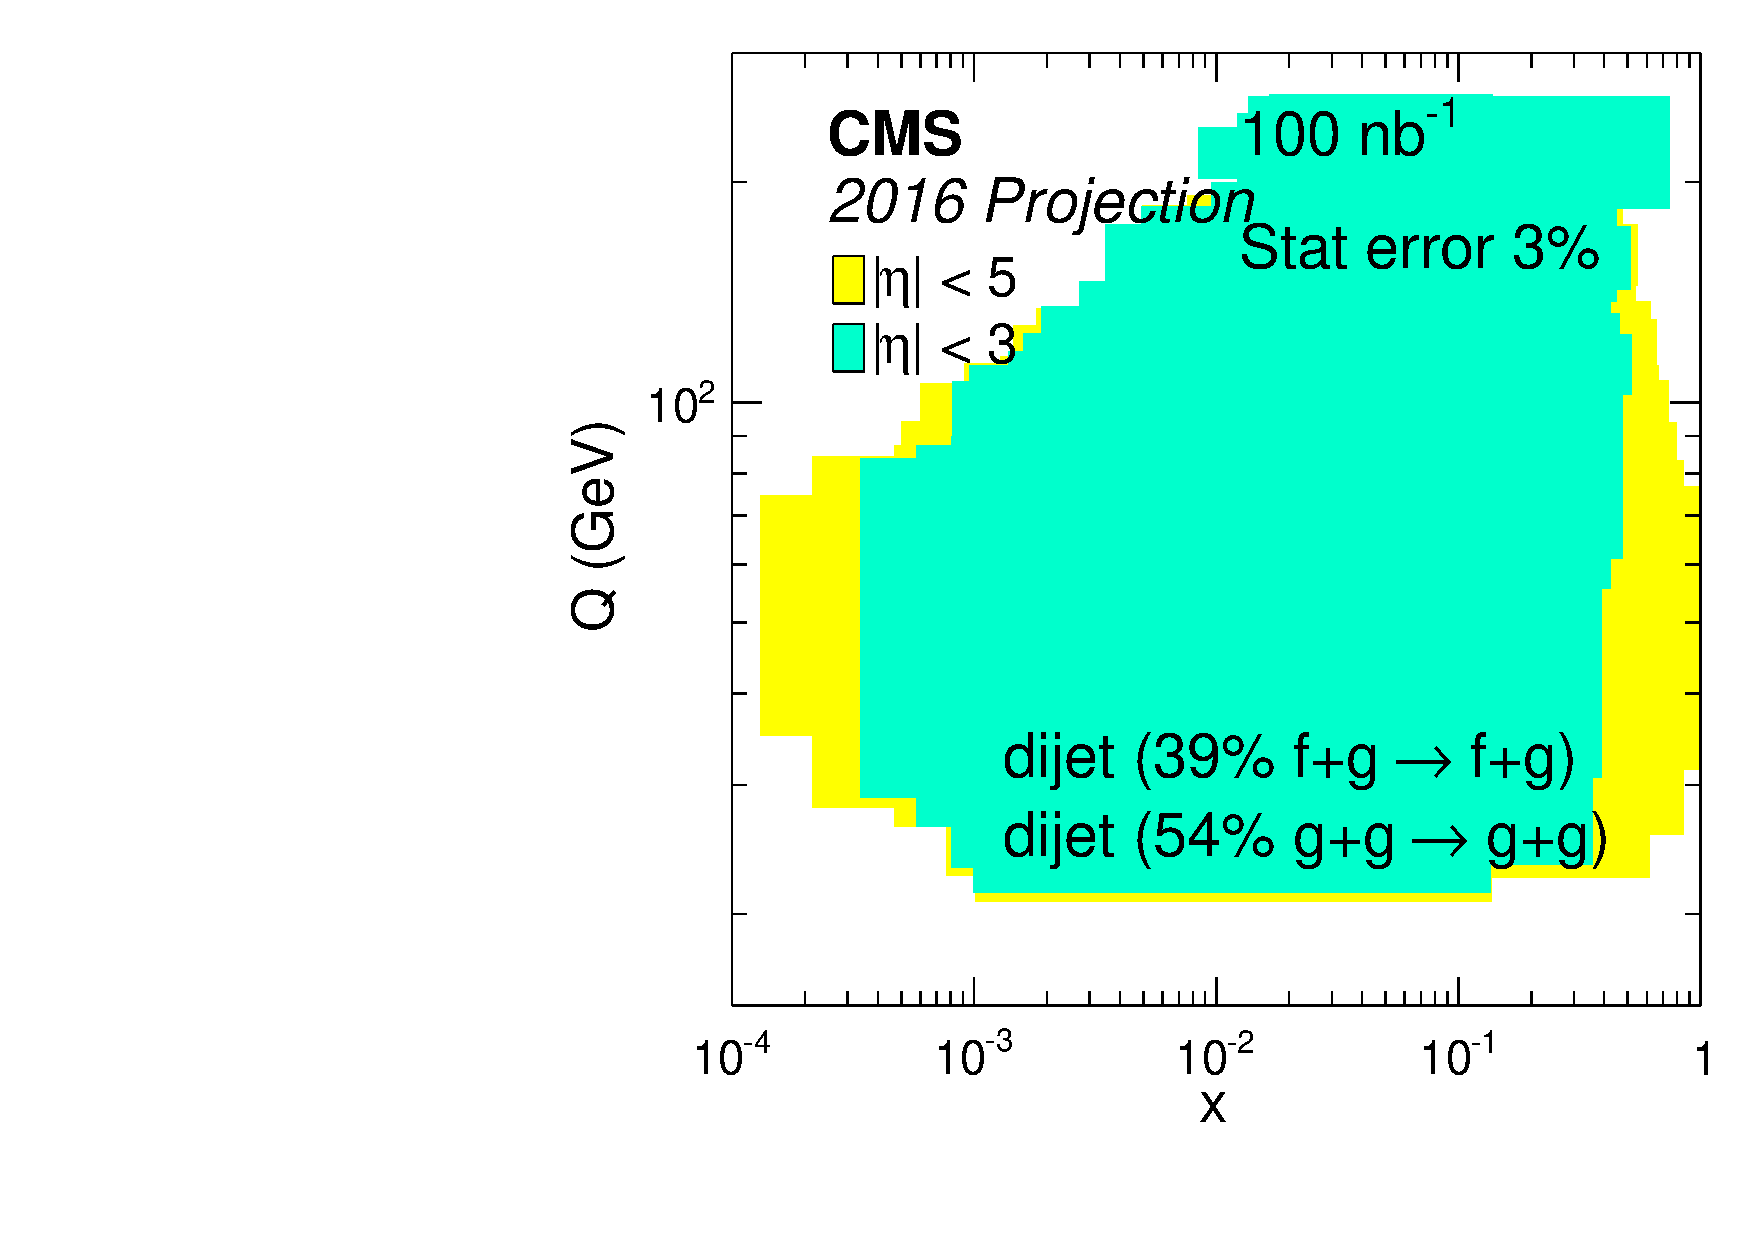
\includegraphics[width= 0.4\textwidth]{figures/filledQX_Lumi100_InclusiveJet_etaComparison.pdf}
\caption{}
\label{fig:xQscanInclusive}
\end{center}
\end{figure}

\begin{figure}[h]
\begin{center}
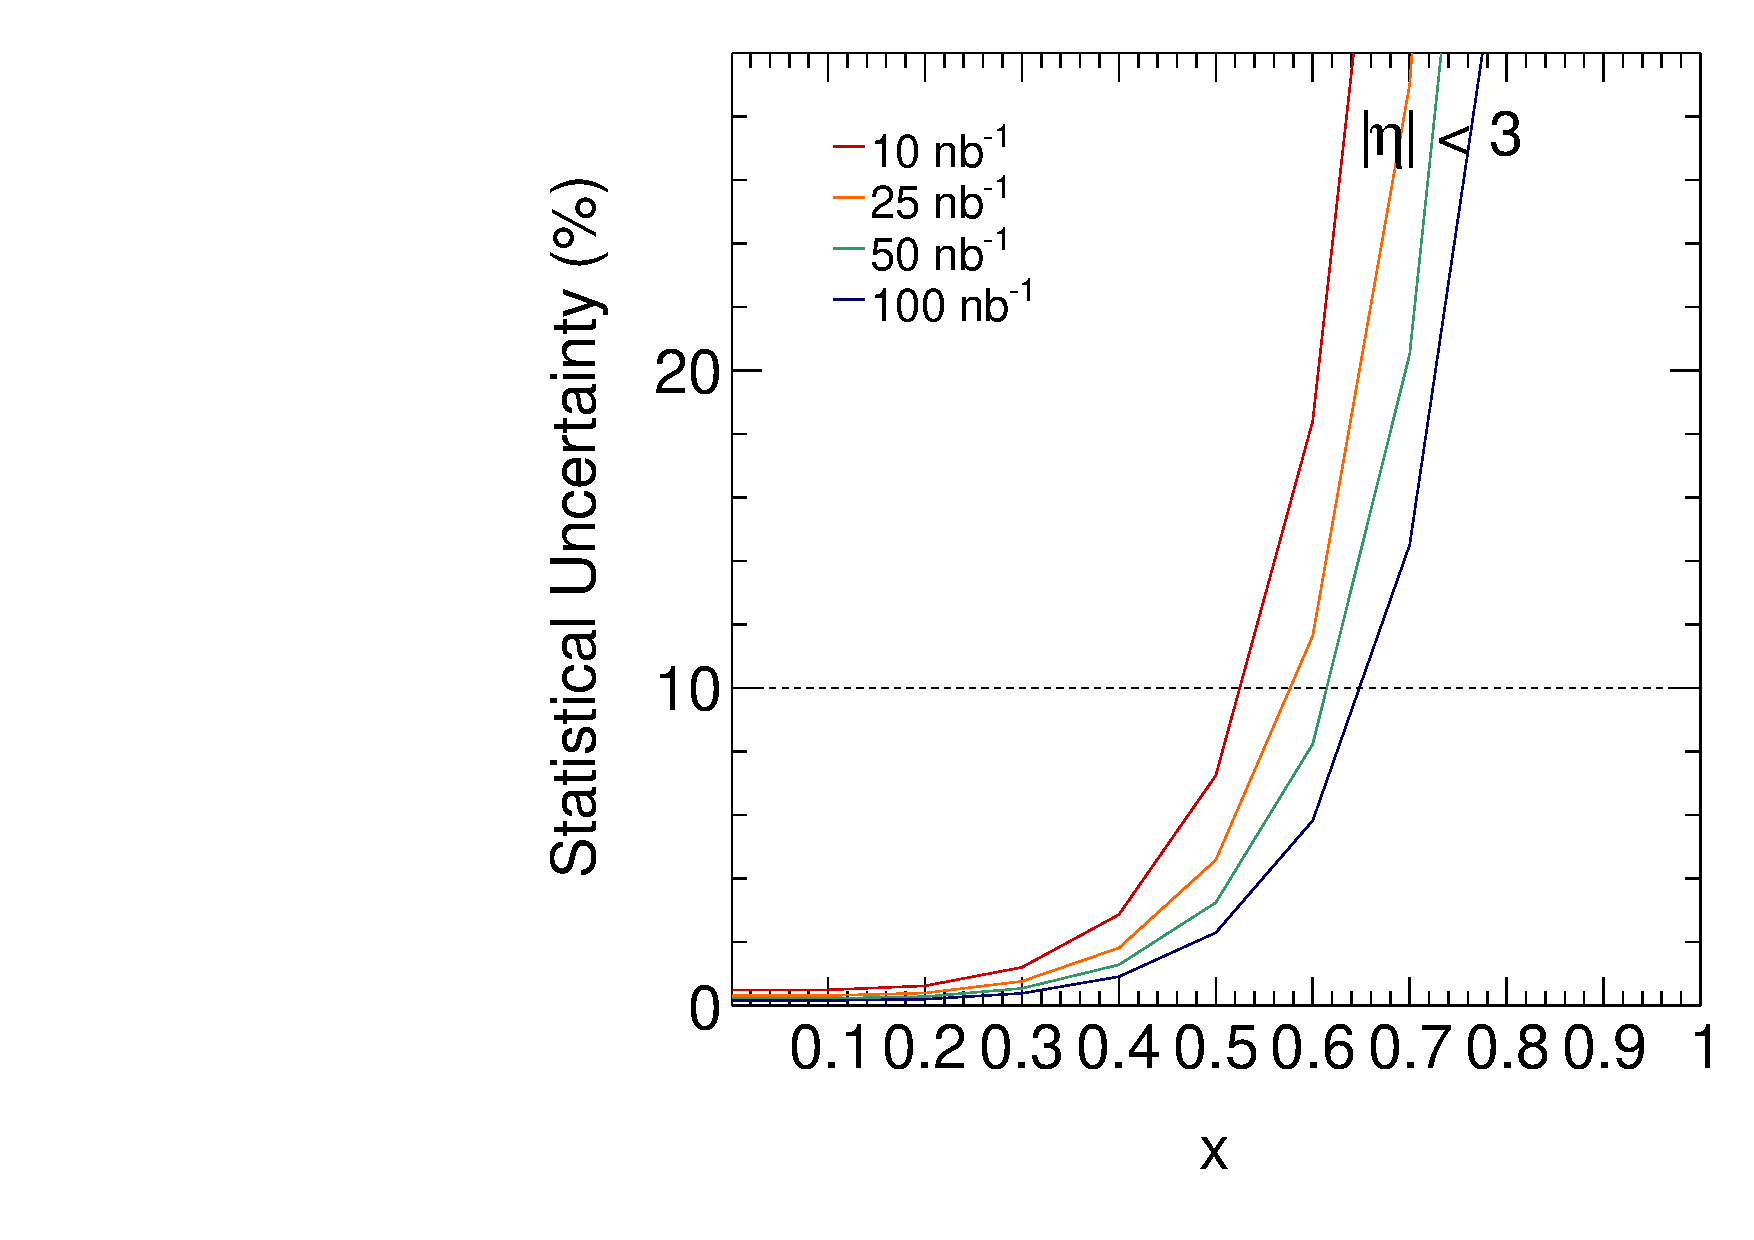
\includegraphics[width= 0.3\textwidth]{figures/xStat_eta3_inclusiveJet.pdf}
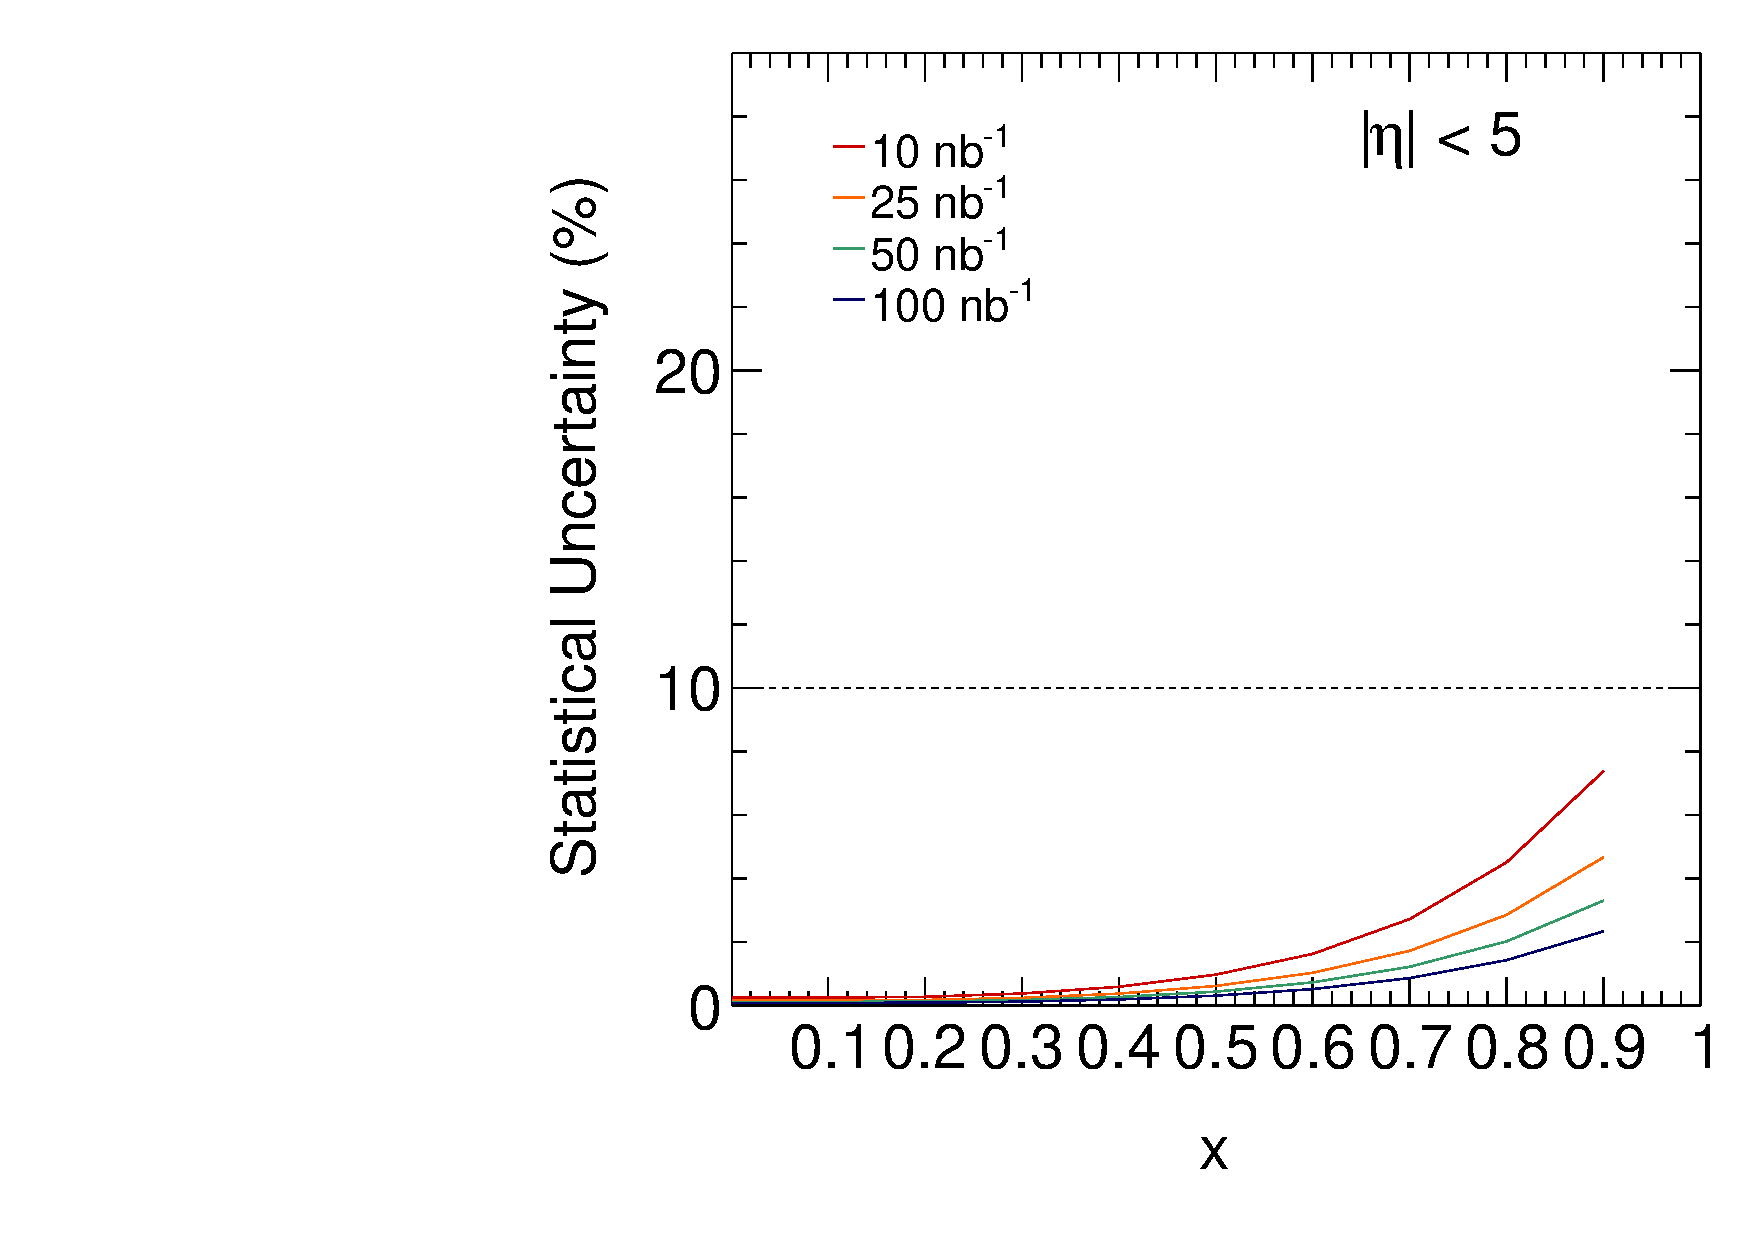
\includegraphics[width= 0.3\textwidth]{figures/xStat_eta5_inclusiveJet.pdf}
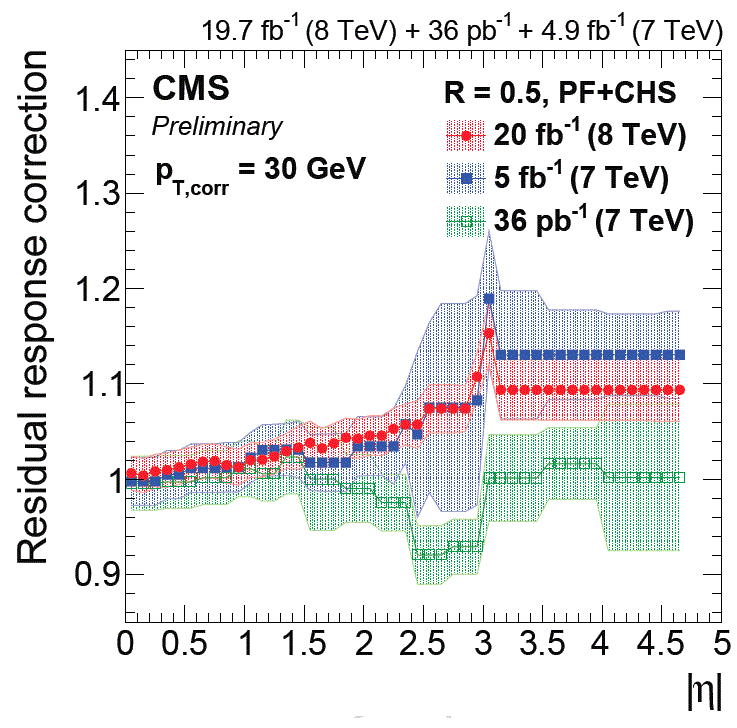
\includegraphics[width= 0.3\textwidth]{figures/staterror_jec_luminosity_pp.png}
\caption{}
\label{fig:XreachWithPseudorapidity}
\end{center}
\end{figure}